% CCI SoM / SoC Selection --- Block Diagrams, Comparison, Cert Mapping
% Document ID: CCLI-SOM-CMP-001  |  Revision 1.0
% Primary SoC datasheet: IMX8MDQLQCEC (i.MX 8M Dual/QuadLite/Quad) Rev. 3
% Build: pdflatex CCI_SoM_Comparison.tex (×2)

\documentclass[10pt,a4paper]{article}

\usepackage[T1]{fontenc}
\usepackage[utf8]{inputenc}
\usepackage{lmodern}
\usepackage{geometry}
\geometry{margin=18mm}

\usepackage{booktabs}
\usepackage{array}
\usepackage{tabularx}
\usepackage{ragged2e}
\usepackage{hyperref}
\usepackage{xcolor}
\usepackage{enumitem}
\usepackage{fancyhdr}
\usepackage{eurosym}
\usepackage{tikz}
\usetikzlibrary{shapes,arrows.meta,positioning,fit,calc}

\hypersetup{
  colorlinks=true,
  linkcolor=blue!60!black,
  urlcolor=blue!60!black,
  pdftitle={CCI SoM Comparison},
  pdfauthor={CCLI}
}

\definecolor{cpuG}{RGB}{120,160,80}
\definecolor{mmO}{RGB}{210,130,60}
\definecolor{ioT}{RGB}{70,140,150}
\definecolor{secB}{RGB}{70,110,170}
\definecolor{sysOl}{RGB}{140,140,60}
\definecolor{memY}{RGB}{200,180,60}
\definecolor{needR}{RGB}{185,28,28}
\definecolor{okG}{RGB}{22,101,52}
\definecolor{warnA}{RGB}{180,83,9}
\definecolor{okbg}{RGB}{240,253,244}
\definecolor{warnbg}{RGB}{255,251,235}
\definecolor{missbg}{RGB}{254,242,242}

\pagestyle{fancy}
\fancyhf{}
\fancyhead[L]{\small CCLI-SOM-CMP-001 rev.\ 1.0}
\fancyhead[R]{\small SoM / SoC Comparison}
\fancyfoot[C]{\thepage}
\renewcommand{\headrulewidth}{0.4pt}

\newcommand{\file}[1]{\texttt{#1}}
\newcommand{\docref}[1]{\textbf{#1}}
\newcommand{\yes}{\textcolor{okG}{\textbf{Yes}}}
\newcommand{\no}{\textcolor{needR}{\textbf{No}}}
\newcommand{\partly}{\textcolor{warnA}{\textbf{Partial}}}

\title{%
  \textbf{CCI Compute Selection --- SoC Block Diagrams \& Comparison}\\[0.35em]
  \large Mapping project I/O needs, security features, and certification scope
}
\author{Document ID: CCLI-SOM-CMP-001 \quad Revision: 1.0\\
Companion to \docref{CCLI-ROADMAP-001}}
\date{2026-07-25}

\begin{document}
\maketitle
\thispagestyle{empty}

\begin{abstract}
\noindent
This document compares every compute option listed in the CCI roadmap against the functional I/O and security needs of a CEI~0-16 Annex~O/T Central Plant Controller.
It includes NXP-style SoC block diagrams for the three relevant i.MX~8M families, a SoM packaging comparison (Toradex / Variscite / Compulab / NXP EVK), a certificate-capability map, and a \textbf{missing-data checklist} required before Architecture Freeze.

\textbf{Primary PDF ingested:} \file{IMX8MDQLQCEC-1280316.pdf} --- NXP i.MX~8M Dual / QuadLite / Quad Applications Processors Data Sheet (Consumer), Rev.~3, 04/2021 (Document Number: IMX8MDQLQCEC).
\end{abstract}

\begin{center}
\begin{minipage}{0.95\linewidth}
\colorbox{warnbg}{%
  \parbox{\dimexpr\linewidth-2\fboxsep\relax}{%
    \small
    \textbf{\textcolor{warnA}{Important naming note:}}
    The PDF you added is the \textbf{i.MX~8M Dual/QuadLite/Quad} family (matches the block-diagram screenshot), \emph{not} i.MX~8M Plus.
    Plus (NPU + Cortex-M7 + dual GbE MAC) is a different SoC --- both appear in the comparison because Toradex/Variscite ship both Mini and Plus SoMs.
  }%
}
\end{minipage}
\end{center}

\tableofcontents
\newpage

%==============================================================================
\section{What the CCI project actually needs from the SoC/SoM}
\label{sec:needs}
%==============================================================================

\begin{table}[htbp]
\centering
\caption{CCI functional needs vs typical SoC contribution}
\label{tab:needs}
\renewcommand{\arraystretch}{1.1}
\small
\begin{tabularx}{\linewidth}{@{}>{\raggedright\arraybackslash}p{3.2cm}>{\RaggedRight\arraybackslash}X>{\raggedright\arraybackslash}p{3.4cm}@{}}
\toprule
\textbf{CCI need} & \textbf{Must come from} & \textbf{SoC alone?} \\
\midrule
Embedded Linux + IEC~61850 + Modbus & Cortex-A53 cluster + Yocto BSP & \yes\ (performance) \\
Real-time / GOOSE assist (optional) & Cortex-M4/M7 co-processor or hard IRQ path & \partly \\
$\geq$4 Ethernet ports (Eth\_A/B + 2 plant) & SoC MAC(s) + \textbf{external switch/PHYs on carrier} & \no\ --- carrier \\
RS-485 $\times$2 isolated & UART/SPI + \textbf{isolated transceivers} & \no\ --- carrier \\
DI 10--120\,Vdc / DO dry contact & GPIO + \textbf{opto/relays} & \no\ --- carrier \\
GNSS time sync & UART/I2C + \textbf{GNSS module}; IEEE~1588 helps & \partly \\
LTE modem (optional) & USB/PCIe/UART + \textbf{modem module} & \no\ --- carrier \\
Secure boot + key storage & HAB/TrustZone + \textbf{external SE recommended} & \partly \\
ATEX (org already certified) & Process/QMS --- not a SoC feature & N/A \\
IEC~62443 / IEC~62351 & Secure boot, crypto, TLS stack + process & \partly \\
IEC~61850 conformance & Software stack + lab test & \no\ --- stack/lab \\
\bottomrule
\end{tabularx}
\end{table}

\noindent
\textbf{Rule of thumb:} pick the SoM for Linux BSP maturity, industrial temp, dual Ethernet MAC (if possible), HAB/secure boot, and 10-year longevity.
The carrier board still owns the CEI field interfaces.

%==============================================================================
\section{SoC family A --- i.MX 8M Dual / QuadLite / Quad}
\label{sec:imx8m}
%==============================================================================

Source: \file{IMX8MDQLQCEC-1280316.pdf} (your PDF). Consumer datasheet Rev.~3.

\subsection{System block diagram (NXP-style)}

\begin{figure}[htbp]
\centering
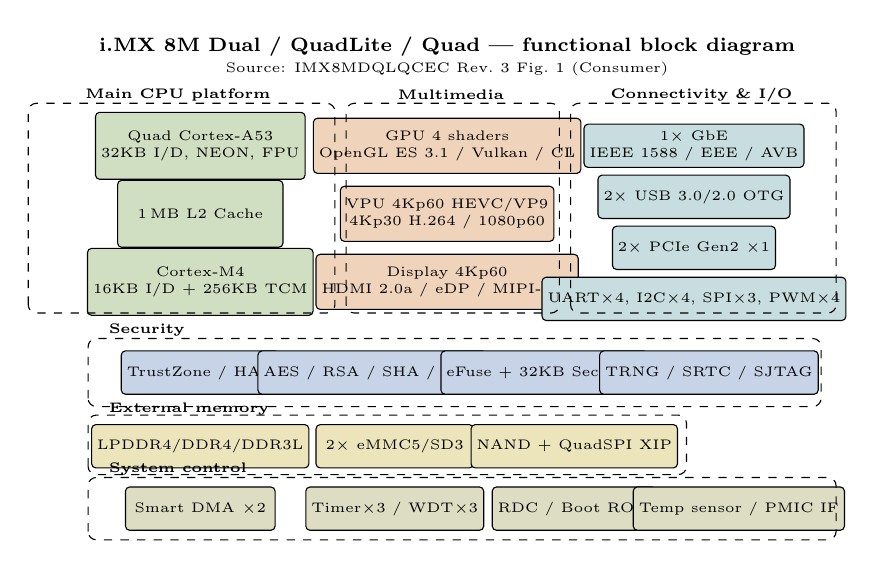
\begin{tikzpicture}[
  x=0.95cm, y=0.72cm,
  box/.style={draw, rounded corners=1.5pt, align=center, font=\tiny, inner sep=2pt},
  cpu/.style={box, fill=cpuG!35, minimum width=2.1cm, minimum height=0.85cm},
  mm/.style={box, fill=mmO!35, minimum width=2.0cm, minimum height=0.7cm},
  io/.style={box, fill=ioT!30, minimum width=2.0cm, minimum height=0.55cm},
  sec/.style={box, fill=secB!30, minimum width=1.9cm, minimum height=0.55cm},
  sys/.style={box, fill=sysOl!30, minimum width=1.9cm, minimum height=0.55cm},
  mem/.style={box, fill=memY!35, minimum width=2.0cm, minimum height=0.55cm},
  title/.style={font=\scriptsize\bfseries}
]

\node[title] at (5.5,8.55) {i.MX 8M Dual / QuadLite / Quad --- functional block diagram};
\node[title, font=\tiny] at (5.5,8.15) {Source: IMX8MDQLQCEC Rev.~3 Fig.~1 (Consumer)};

% CPU
\node[cpu] (a53) at (2.2,6.8) {Quad Cortex-A53\\32KB I/D, NEON, FPU};
\node[cpu] (l2) at (2.2,5.6) {1\,MB L2 Cache};
\node[cpu] (m4) at (2.2,4.4) {Cortex-M4\\16KB I/D + 256KB TCM};

% Multimedia
\node[mm] (gpu) at (5.5,6.8) {GPU 4 shaders\\OpenGL ES 3.1 / Vulkan / CL};
\node[mm] (vpu) at (5.5,5.6) {VPU 4Kp60 HEVC/VP9\\4Kp30 H.264 / 1080p60};
\node[mm] (disp) at (5.5,4.4) {Display 4Kp60\\HDMI 2.0a / eDP / MIPI-DSI};

% Connectivity
\node[io] (eth) at (8.8,6.8) {1$\times$ GbE\\IEEE~1588 / EEE / AVB};
\node[io] (usb) at (8.8,5.9) {2$\times$ USB 3.0/2.0 OTG};
\node[io] (pcie) at (8.8,5.0) {2$\times$ PCIe Gen2 $\times$1};
\node[io] (uart) at (8.8,4.1) {UART$\times$4, I2C$\times$4, SPI$\times$3, PWM$\times$4};

% Security
\node[sec] (tz) at (2.2,2.8) {TrustZone / HAB};
\node[sec] (crypto) at (4.5,2.8) {AES / RSA / SHA / ECC};
\node[sec] (efuse) at (6.8,2.8) {eFuse + 32KB SecRAM};
\node[sec] (rng) at (9.0,2.8) {TRNG / SRTC / SJTAG};

% Memory
\node[mem] (ddr) at (2.2,1.5) {LPDDR4/DDR4/DDR3L};
\node[mem] (emmc) at (4.8,1.5) {2$\times$ eMMC5/SD3};
\node[mem] (nand) at (7.2,1.5) {NAND + QuadSPI XIP};

% System
\node[sys] (dma) at (2.2,0.4) {Smart DMA $\times$2};
\node[sys] (wdg) at (4.8,0.4) {Timer$\times$3 / WDT$\times$3};
\node[sys] (rdc) at (7.2,0.4) {RDC / Boot ROM};
\node[sys] (temp) at (9.4,0.4) {Temp sensor / PMIC IF};

\draw[dashed, rounded corners=3pt] (-0.1,3.85) rectangle (4.0,7.55);
\node[font=\tiny\bfseries] at (1.9,7.7) {Main CPU platform};
\draw[dashed, rounded corners=3pt] (4.15,3.85) rectangle (7.0,7.55);
\node[font=\tiny\bfseries] at (5.55,7.7) {Multimedia};
\draw[dashed, rounded corners=3pt] (7.15,3.85) rectangle (10.7,7.55);
\node[font=\tiny\bfseries] at (8.9,7.7) {Connectivity \& I/O};
\draw[dashed, rounded corners=3pt] (0.7,2.2) rectangle (10.5,3.4);
\node[font=\tiny\bfseries, anchor=west] at (0.85,3.55) {Security};
\draw[dashed, rounded corners=3pt] (0.7,1.0) rectangle (8.7,2.05);
\node[font=\tiny\bfseries, anchor=west] at (0.85,2.15) {External memory};
\draw[dashed, rounded corners=3pt] (0.7,-0.15) rectangle (10.7,0.95);
\node[font=\tiny\bfseries, anchor=west] at (0.85,1.1) {System control};

\end{tikzpicture}
\caption{i.MX 8M Dual/QuadLite/Quad --- reconstructed from IMX8MDQLQCEC Fig.~1}
\label{fig:imx8m-quad}
\end{figure}

\subsection{CCI relevance}

\begin{itemize}[noitemsep]
  \item \textbf{Strength:} full HAB/TrustZone/crypto, Cortex-M4, IEEE~1588 GbE, mature Yocto ecosystem.
  \item \textbf{Gap for CCI:} only \textbf{one} on-chip GbE MAC --- carrier needs Ethernet switch + more PHYs for 4 ports.
  \item \textbf{Caution:} your PDF is the \textbf{Consumer} electricals document --- for utility product you need the \textbf{Industrial} orderable parts and temperature grade confirmation.
\end{itemize}

%==============================================================================
\section{SoC family B --- i.MX 8M Mini}
\label{sec:mini}
%==============================================================================

Used by: Toradex Verdin iMX8M Mini, Variscite DART-MX8M-MINI.

\begin{figure}[htbp]
\centering
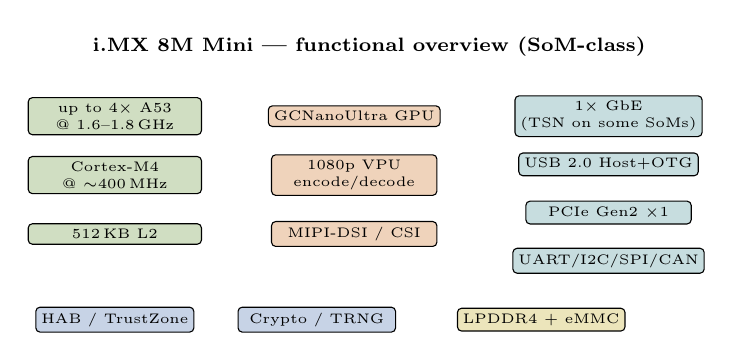
\begin{tikzpicture}[
  x=0.95cm, y=0.68cm,
  box/.style={draw, rounded corners=1.5pt, align=center, font=\tiny, inner sep=2pt},
  cpu/.style={box, fill=cpuG!35, minimum width=2.2cm},
  mm/.style={box, fill=mmO!35, minimum width=2.1cm},
  io/.style={box, fill=ioT!30, minimum width=2.1cm},
  sec/.style={box, fill=secB!30, minimum width=2.0cm},
  mem/.style={box, fill=memY!35, minimum width=2.0cm},
  title/.style={font=\scriptsize\bfseries}
]
\node[title] at (5.2,6.3) {i.MX 8M Mini --- functional overview (SoM-class)};
\node[cpu] at (1.8,5.0) {up to 4$\times$ A53\\@ 1.6--1.8\,GHz};
\node[cpu] at (1.8,3.9) {Cortex-M4\\@ $\sim$400\,MHz};
\node[cpu] at (1.8,2.8) {512\,KB L2};
\node[mm] at (5.0,5.0) {GCNanoUltra GPU};
\node[mm] at (5.0,3.9) {1080p VPU\\encode/decode};
\node[mm] at (5.0,2.8) {MIPI-DSI / CSI};
\node[io] at (8.4,5.0) {1$\times$ GbE\\(TSN on some SoMs)};
\node[io] at (8.4,4.1) {USB 2.0 Host+OTG};
\node[io] at (8.4,3.2) {PCIe Gen2 $\times$1};
\node[io] at (8.4,2.3) {UART/I2C/SPI/CAN};
\node[sec] at (1.8,1.2) {HAB / TrustZone};
\node[sec] at (4.5,1.2) {Crypto / TRNG};
\node[mem] at (7.5,1.2) {LPDDR4 + eMMC};
\end{tikzpicture}
\caption{i.MX 8M Mini --- simplified SoC block overview}
\label{fig:imx8m-mini}
\end{figure}

\noindent
\textbf{CCI fit:} usually enough CPU for IEC~61850 + Modbus; lower cost/power than Plus/Quad; still needs external Ethernet switch for 4 ports; weaker multimedia (irrelevant for CCI).

%==============================================================================
\section{SoC family C --- i.MX 8M Plus}
\label{sec:plus}
%==============================================================================

Used by: Toradex Verdin iMX8M Plus, Variscite DART-MX8M-PLUS.

\begin{figure}[htbp]
\centering
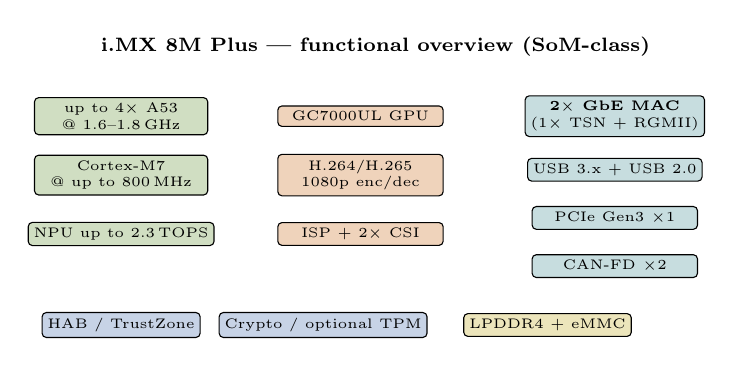
\begin{tikzpicture}[
  x=0.95cm, y=0.68cm,
  box/.style={draw, rounded corners=1.5pt, align=center, font=\tiny, inner sep=2pt},
  cpu/.style={box, fill=cpuG!35, minimum width=2.2cm},
  mm/.style={box, fill=mmO!35, minimum width=2.1cm},
  io/.style={box, fill=ioT!30, minimum width=2.1cm},
  sec/.style={box, fill=secB!30, minimum width=2.0cm},
  mem/.style={box, fill=memY!35, minimum width=2.0cm},
  title/.style={font=\scriptsize\bfseries}
]
\node[title] at (5.2,6.5) {i.MX 8M Plus --- functional overview (SoM-class)};
\node[cpu] at (1.8,5.2) {up to 4$\times$ A53\\@ 1.6--1.8\,GHz};
\node[cpu] at (1.8,4.1) {Cortex-M7\\@ up to 800\,MHz};
\node[cpu] at (1.8,3.0) {NPU up to 2.3\,TOPS};
\node[mm] at (5.0,5.2) {GC7000UL GPU};
\node[mm] at (5.0,4.1) {H.264/H.265\\1080p enc/dec};
\node[mm] at (5.0,3.0) {ISP + 2$\times$ CSI};
\node[io] at (8.4,5.2) {\textbf{2$\times$ GbE MAC}\\(1$\times$ TSN + RGMII)};
\node[io] at (8.4,4.2) {USB 3.x + USB 2.0};
\node[io] at (8.4,3.3) {PCIe Gen3 $\times$1};
\node[io] at (8.4,2.4) {CAN-FD $\times$2};
\node[sec] at (1.8,1.3) {HAB / TrustZone};
\node[sec] at (4.5,1.3) {Crypto / optional TPM};
\node[mem] at (7.5,1.3) {LPDDR4 + eMMC};
\end{tikzpicture}
\caption{i.MX 8M Plus --- simplified SoC block overview}
\label{fig:imx8m-plus}
\end{figure}

\noindent
\textbf{CCI fit:} \textbf{best Ethernet story} --- two MAC ports on-chip (still need a switch/PHY strategy for 4 external RJ45s, but Eth\_A/Eth\_B isolation is easier). M7 is a stronger real-time co-processor than M4. NPU is unused for CCI (cost you may not need).

%==============================================================================
\section{SoM packaging comparison (roadmap choices)}
\label{sec:som-table}
%==============================================================================

\begin{table}[htbp]
\centering
\caption{Roadmap SoM options --- comparison for CCI carrier design}
\label{tab:som}
\renewcommand{\arraystretch}{1.12}
\footnotesize
\begin{tabularx}{\linewidth}{@{}>{\raggedright\arraybackslash}p{2.5cm}cccc>{\RaggedRight\arraybackslash}X@{}}
\toprule
\textbf{Option} & \textbf{SoC} & \textbf{GbE} & \textbf{RT core} & \textbf{Ind.\ temp} & \textbf{CCI notes} \\
\midrule
Toradex Verdin iMX8M Mini &
8M Mini &
1 (+TSN) &
M4 &
Yes (IT SKUs) &
Pin-compatible Verdin; strong Torizon/Yocto; good cost. \\
Toradex Verdin iMX8M Plus &
8M Plus &
\textbf{2} &
M7 &
Yes (IT SKUs) &
Best Ethernet; optional Wi-Fi/BT \emph{not needed} for CCI; optional TPM. \\
Variscite DART-MX8M-MINI &
8M Mini &
1 &
M4 &
Yes &
Compact DART pin2pin; certified Wi-Fi SKUs available (unused for CCI). \\
Variscite DART-MX8M-PLUS &
8M Plus &
\textbf{2} &
M7 &
Yes &
Dual GbE + CAN-FD; pin2pin with Mini. \\
Compulab CL-SOM-iMX8 &
8M Dual/Quad class &
1 typ. &
M4 &
Check SKU &
Confirm exact SoC variant + longevity with Compulab. \\
NXP i.MX8M EVK / bare SoC &
8M Dual/Quad (your PDF) &
1 &
M4 &
Consumer DS only &
Reference for schematic/layout rules; not a DIN-rail SoM. \\
\bottomrule
\end{tabularx}
\end{table}

\begin{table}[htbp]
\centering
\caption{Carrier I/O impact by SoM choice}
\label{tab:carrier}
\renewcommand{\arraystretch}{1.1}
\small
\begin{tabularx}{\linewidth}{@{}>{\raggedright\arraybackslash}p{3.0cm}>{\RaggedRight\arraybackslash}X>{\RaggedRight\arraybackslash}X@{}}
\toprule
\textbf{Carrier block} & \textbf{Mini / Dual-Quad (1 MAC)} & \textbf{Plus (2 MAC)} \\
\midrule
Eth\_A (DSO) + Eth\_B (Operator) &
Need managed switch or multi-PHY + VLAN/isolation design carefully &
Can attach DSO and Operator to separate MACs --- cleaner isolation story \\
2$\times$ plant Ethernet &
External switch ports &
External switch ports (same) \\
RS-485 $\times$2, DI/DO, GNSS, LTE &
Identical --- all on carrier &
Identical --- all on carrier \\
Secure element &
External SE recommended on both &
External SE; Plus SKUs may add TPM \\
\bottomrule
\end{tabularx}
\end{table}

%==============================================================================
\section{Certificates --- what the silicon helps with vs what you still buy}
\label{sec:certs}
%==============================================================================

\begin{table}[htbp]
\centering
\caption{Certification workstreams vs SoC/SoM contribution}
\label{tab:certs}
\renewcommand{\arraystretch}{1.12}
\small
\begin{tabularx}{\linewidth}{@{}>{\raggedright\arraybackslash}p{2.8cm}>{\RaggedRight\arraybackslash}X>{\raggedright\arraybackslash}p{2.6cm}@{}}
\toprule
\textbf{Certificate / requirement} & \textbf{What SoC/SoM can handle} & \textbf{Still needed} \\
\midrule
\textbf{ATEX} (EN/IEC~60079) &
Nothing silicon-specific for a typical non-Ex MT cabinet CCI &
\textbf{Already held by org} --- reuse QMS/NB \\
IEC~62443-4-1 (SDLC) &
HAB secure-boot docs, signed images, SBOM habits &
Process audit, threat model, patch policy \\
IEC~62443-4-2 (device) &
TrustZone, crypto accel, secure RAM, optional TPM &
Lab test, RBAC, audit log, hardened OS image \\
IEC~62351 &
HW crypto for TLS/DTLS performance &
Protocol stack + scarce lab capacity \\
IEC~61850 conformance &
CPU performance only &
libiec61850 or commercial stack + lab \\
CEI~0-16 Annex~O/T &
Interfaces + time sync (1588/GNSS) &
DSO demo, PF2 logic, functional evidence \\
EMC / electrical safety &
SoM vendor industrial design guides help &
Carrier layout + type tests \\
Radio (if LTE/Wi-Fi used) &
Some SoMs ship pre-certified Wi-Fi modules &
LTE module RED/FCC; antenna design \\
\bottomrule
\end{tabularx}
\end{table}

\begin{center}
\begin{minipage}{0.95\linewidth}
\colorbox{okbg}{%
  \parbox{\dimexpr\linewidth-2\fboxsep\relax}{%
    \small
    \textbf{\textcolor{okG}{Recommendation (engineering default):}}
    Prefer an \textbf{i.MX~8M Plus} SoM (Toradex Verdin or Variscite DART) \textbf{Industrial} grade for dual GbE MAC + M7.
    Drop Wi-Fi SKU unless you need it. Keep external secure element.
    Mini remains valid if BOM must stay near the low end of the \EUR{}60--120 SoM band.
  }%
}
\end{minipage}
\end{center}

%==============================================================================
\section{Missing data --- required before Architecture Freeze}
\label{sec:missing}
%==============================================================================

\begin{center}
\begin{minipage}{0.95\linewidth}
\colorbox{missbg}{%
  \parbox{\dimexpr\linewidth-2\fboxsep\relax}{%
    \small
    \textbf{\textcolor{needR}{Stop-ship for schematic:}}
    the items below are not yet in the CCLI corpus (or are wrong/incomplete). Fill these to freeze connectors, power budget, and SoM SKU.
  }%
}
\end{minipage}
\end{center}

\subsection{Critical (block schematic / pin budget)}

\begin{enumerate}[leftmargin=*]
  \item \textbf{Final SoM SKU} --- vendor + exact P/N (RAM/eMMC/temp grade/Wi-Fi yes-no/TPM yes-no).
  \item \textbf{Industrial vs Consumer SoC grade} --- your IMX8MDQLQCEC PDF is Consumer; need Industrial datasheet or SoM datasheet for $-40$ to $+85\,^\circ$C SKU.
  \item \textbf{Ethernet architecture decision} --- 4-port managed switch IC vs SoM dual-MAC + 2-port switch; VLAN vs physically isolated PHYs for Eth\_A.
  \item \textbf{Energy analyzer interface} --- exact Modbus map / baud / RS-485 bias for the analyzer you will use (Ax M22/MT1-class or real P/N).
  \item \textbf{DI/DO count and voltage classes} --- how many DI channels, DO relays, and whether PF2 is single or dual DO.
  \item \textbf{Power budget} --- 12--24\,Vdc input current at boot + LTE TX peak; SoM + switch + modem peaks.
  \item \textbf{Real STM32 datasheet} --- \file{STM32L151RCTx.pdf} in the folder is a \textbf{duplicate of the AiLux CCI manual}, not an STM32 PDF. Replace or delete.
\end{enumerate}

\subsection{Important (cert / firmware / procurement)}

\begin{enumerate}[leftmargin=*, resume]
  \item \textbf{ATEX certificate scope text} --- certificate number, product family covered, QAN --- so we can cite it precisely in \docref{CCLI-ROADMAP-001}.
  \item \textbf{IEC~61850 stack decision} --- stay on libiec61850 for prototype or budget commercial stack now.
  \item \textbf{Target security level} --- SL1 vs SL2 for 62443-4-2 (drives lab quote).
  \item \textbf{Longevity / PCN commitment letters} --- Toradex / Variscite / Compulab 10-year statements for chosen SKU.
  \item \textbf{Compulab CL-SOM-iMX8 exact datasheet} --- not yet in RAG; needed if that vendor stays in shortlist.
  \item \textbf{i.MX 8M Mini and 8M Plus NXP datasheets} --- only Dual/Quad Consumer PDF is present; add Mini + Plus (Industrial) PDFs for complete block-level parity.
  \item \textbf{Secure element P/N} --- ATECC608B vs STSAFE-A110 (or TPM on Plus SoM) decision.
\end{enumerate}

\subsection{Nice-to-have}

\begin{enumerate}[leftmargin=*, resume]
  \item Carrier mechanical envelope (DIN-rail width / height / depth).
  \item DSO FO media-converter preference (external SFP vs onboard).
  \item Whether LTE is required on rev~A or deferred.
\end{enumerate}

%==============================================================================
\section{Documents in corpus / RAG status}
\label{sec:rag}
%==============================================================================

\begin{tabularx}{\linewidth}{@{}>{\raggedright\arraybackslash}p{4.2cm}l>{\RaggedRight\arraybackslash}X@{}}
\toprule
\textbf{File} & \textbf{RAG source\_id} & \textbf{Status} \\
\midrule
IMX8MDQLQCEC-1280316.pdf & \texttt{ccli-nxp-imx8m-dqlq-cec} & Ingest this revision \\
CCI\_Project\_Roadmap.md/.pdf & \texttt{ccli-project-roadmap} & Re-ingest after ATEX/Altium edits \\
CCI\_SoM\_Comparison (this doc) & \texttt{ccli-som-comparison} & Ingest after PDF build \\
CCI\_Clone\_RE\_Option.pdf & \texttt{ccli-clone-re-option} & Optional ingest \\
Toradex / Variscite datasheets & --- & \textbf{Missing --- add PDFs} \\
i.MX 8M Mini / Plus NXP DS & --- & \textbf{Missing} \\
Real STM32L151 datasheet & --- & \textbf{Missing (current file is wrong)} \\
\bottomrule
\end{tabularx}

%==============================================================================
\section{Immediate next actions}
%==============================================================================

\begin{enumerate}[leftmargin=*]
  \item Decide shortlist of \textbf{two} SoMs (recommended: Verdin Plus IT vs DART-MX8M-PLUS IT).
  \item Drop the matching vendor SoM PDF into the CCLI project folder and we will RAG + extract pinout.
  \item Provide ATEX certificate PDF or number/scope.
  \item Replace the misnamed STM32 PDF.
  \item Then draft \textbf{CCLI-IF-001} connector/pin-budget from the winner SoM datasheet.
\end{enumerate}

\end{document}
